%%%%%%%%%%%%%%%%%%%%%%%%%%%%%%%%%%%%%%%%%%%%%%%%%%%%%%%%%%%%%%%%%%%%%%%%%%%
% Definitions                                                             %
%%%%%%%%%%%%%%%%%%%%%%%%%%%%%%%%%%%%%%%%%%%%%%%%%%%%%%%%%%%%%%%%%%%%%%%%%%%
\gdef\version{0.1}
\gdef\doctype{Businessplan}

\documentclass[11pt]{article}
%Gummi|065|=)
\usepackage{graphicx}
\usepackage{color}
\usepackage[dvipsnames]{xcolor}
\usepackage{tabu}
\usepackage{fancyhdr}
\usepackage{titlesec}
\usepackage{lastpage}
\usepackage[utf8]{inputenc}
\usepackage{eurosym}

% headers
\renewcommand{\headrulewidth}{0.4pt}
\renewcommand{\footrulewidth}{0.4pt}
\fancyhead{}
\fancyfoot{}
\pagestyle{fancy}
\lhead{{\doctype}}
\rhead{{\fontfamily{phv}\selectfont \textcolor{gray}{Urban Green}} 
\includegraphics[height=0.8cm]{logo}}
\lfoot{Version \version}
\rfoot{\thepage\ von \pageref{LastPage}}
\setlength{\headheight}{30pt}

%%%%%%%%%%%%%%%%%%%%%%%%%%%%%%%%%%%%%%%%%%%%%%%%%%%%%%%%%%%%%%%%%%%%%%%%%%%
% Document Start                                                          %
%%%%%%%%%%%%%%%%%%%%%%%%%%%%%%%%%%%%%%%%%%%%%%%%%%%%%%%%%%%%%%%%%%%%%%%%%%%

\begin{document}

\begin{titlepage}
    \centering
    \vfill
    {
        \Huge\textbf{Businessplan}\\
        \vskip2cm
        
\includegraphics[width=4cm]{logo} \\
        \Large 
        {\fontfamily{phv}\selectfont 
			\textcolor{gray}{Urban Green}%
		}
        \vskip3cm
        Matthias Schwebler\\
        Ramin Bahadoorifar\\
        Samuel Schober\\
        Konrad Kelc\\
    }    
    \vfill
    \begin{center}
    \begin{table}[ht]
    	\centering
    	\begin{tabular}{lllll}
    		\cline{1-4}
    		\multicolumn{1}{|c|}{\textbf{\rule{0pt}{3ex} }} & \multicolumn{1}{c|}{\textbf{Name}} & \multicolumn{1}{l|}{\textbf{Datum}} & \multicolumn{1}{l|}{\textbf{Unterschrift}} &  \\ \cline{1-4}
    		
    		\multicolumn{1}{|l|}{\textbf{\rule{0pt}{3ex} Erstellt:}} & \multicolumn{1}{l|}{M. Schwebler, R. Bahadoorifar} & \multicolumn{1}{l|}{2.11.2016} & \multicolumn{1}{l|}{} &  \\ \cline{1-4}
    		
    		\multicolumn{1}{|l|}{\textbf{\rule{0pt}{3ex} Gepr\"uft:}} & \multicolumn{1}{l|}{S. Schober, K. Kelc} & \multicolumn{1}{l|}{2.11.2016} & \multicolumn{1}{l|}{} &  \\ \cline{1-4}
    		&  &  &  &  \\
    		&  &  &  &  \\
    		&  &  &  &  \\
    		&  &  &  &  \\
    		&  &  &  &  \\
    		&  &  &  & 
    	\end{tabular}
    \end{table}
    \end{center}
\end{titlepage}

\section{Executive Summary}
\section{Produktidee}
\subsection{Kundenbed\"urfnisse und Probleml\"osung}
Urban Green, bietet in \"Osterreich die bisher nicht erh\"altlichen Produkte aus dem Hydroponik Bereich f\"ur den durchschnittlichen Haushalt. Der Kunde kann ein Aquaponic System, welches sonst nur in Betrieben im
großen Ausmaß, durchgef\"uhrt wird, bei sich zuhause hobbym\"aßig betreiben. Dies kann man von den bereits bestehenden Heiml\"osungen nicht behaupten: Sie sind entweder gesetzlich nicht erlaubt oder in \"Osterreich nicht erh\"altlich.\\
\\ Das System bietet eine vollst\"andige \"Uberwachung des Ecosystems, mithilfe von PH-, EC- und Temperatursensoren. Des Weiteren kann das System vom Benutzer gesteuert werden, indem er Aktoren (Hitzestrahler, Futterautomat und Beleuchtung) \"uber die Weboberfl\"ache steuert. \\
\\ \"Uber die Webapp, kann der Benutzer alle Daten der bisher genannten Sensoren und dessen Interpretationen ablesen und gegebenenfalls \"uber Steuerung der Aktoren Maßnahmen ergreifen. \"Uber die Webapp soll der Benutzer auch, bevor er sein Aquaponic System Fischen best\"uckt, ein breites Spektrum an Informationen \"uber m\"ogliche Kombinationen erhalten um eine, f\"ur ihn, optimale Besetzung des Aquariums und des Beetes zu erzielen. Er soll auch eigene "Profile" erstellen k\"onnen und andere Bewerten k\"onnen. So w\"achst das Portal, lediglich durch die Verwendung der Benutzer.
\newpage
\subsection{Produkte und Dienstleistungen}
Das Endprodukt ist ein Aquaponic System (Aquarium + Beet f\"ur Anbau), welches \"uber eine Website \"uberwacht bzw. gesteuert werden kann. Dazu z\"ahlen Daten wie: Wassertemperatur, EC-Wert, PH-Wert, Wasserstand, Belichtungsdauer und Intensit\"at der Beleuchtung.
\begin{center}
	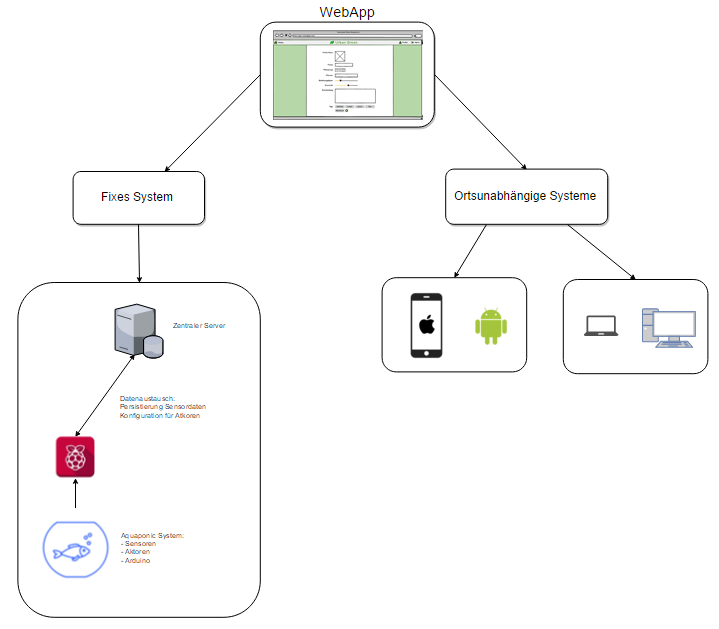
\includegraphics[width=12cm]{produkte}
\end{center}
\subsubsection{WebApp}
Besitzer eines Urban Green Aquaponic Systems, bekommen alle Daten der Sensoren in aufbereiteter Form, auf der WebApp zur Verf\"ugung gestellt. \"Uber die Website kann aber nicht nur abgelesen werden, sondern auch Konfigurationen f\"ur die Aktoren angepasst werden. \\
Neben den Echtzeitinformationen, k\"onnen auch Erfahrungswerte anderer Benutzer, bez\"uglich der Kombinationen von Fisch und Pflanzen gelesen und bewertet werden. So w\"achst das Portal stetig durch die Benutzung der Kunden. \\
Da das Produkt f\"ur die Marktl\"ucke in \"Osterreich und Deutschland konzipiert ist, wird die Website vorerst nur in Deutsch betrieben. 
\subsubsection{Fixes System}
Das Aquarium und das Beet stellen das fixe System dar. Enthalten sind: Sensoren, Aktoren sowie ein Arduino und ein Raspberry Pi. Der Arduino \"ubernimmt die Schnittstelle zu den Sensoren. Er sendet in regelm\"aßigen Abst\"anden die Daten aller Sensoren an den Raspberry Pi und \"andert die Werte f\"ur die Aktoren (falls neue Konfiguration des Benutzers vorhanden). Der Raspberry Pi \"ubernimmt die sichere Kommunikation mit einem zentralen Server. Er sendet die Daten und fragt gleichzeitig neue Konfigurationen f\"ur die Aktoren ab. Sollte der Server nicht erreichbar sein, speichert er die Daten lokal zwischen, und \"ubertr\"agt sie bei Wiederherstellung der Verbindung. 
\begin{center}
	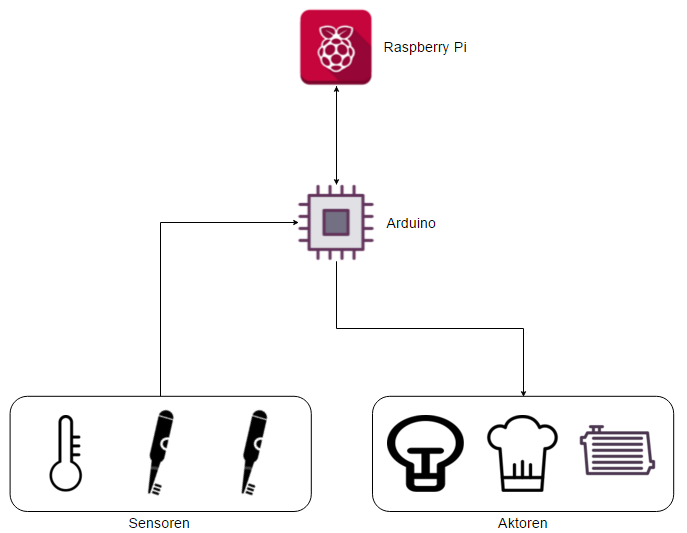
\includegraphics[width=8cm]{fixesSystem}
\end{center}
\vskip1cm
\begin{itemize}
	\item \textbf{Raspberry Pi}: Kommunikation mit Server, Zwischenspeicherung bei Netzausfall 
	\item \textbf{Arduino}: Ansteuerung der Sensoren und Aktoren, \"Ubertragung der Daten an den Raspberry Pi
	\item \textbf{Sensoren}: Temperatur, PH-Wert, EC-Wert, Wasserstand
	\item \textbf{Aktoren}: Beleuchtung der Pflanzen, Futterautomat, Hitzestrahler
\end{itemize}
\subsubsection{Ortsunabh\"angige Systeme}
Da mobile Ger\"ate mittlerweile so verbreitet sind, dass sie bei nahezu jedem anzutreffen sind, wird ist die Schnittstelle des Systems zum Benutzer eine Website. Dies bietet den Vorteil, dass nur eine Applikation erstellt werden muss, die sowohl auf PCs, Laptops und Smartphones funktioniert. So kann der Benutzer auch, weit weg von zuhause auf sein Aquponik System zugreifen. 
\subsection{Einzigartigkeit in \"Osterreich}
Aquaponic Systeme sind haupts\"achlich im gr\"o{\ss}eren Ma{\ss}stab bei der Aufzucht von Nutzpflanzen im Einsatz. F\"ur den normalen Haushalt gibt es allerdings bis jetzt keine Marktf\"ahige L\"osung. Die gr\"o{\ss}ten zwei Crowdfunding Projekte sind:
\begin{itemize}
	\item \textbf{EcoQube C}\\
	Der EcoQube C vereint ein Handliches Aquaponics System mit elegantem Design, jedoch mangelt es an Konfigurierbarkeit. Es steht lediglich eine Fernbedienung zur verf\"ugung, mit der die Farbe der LEDs gesteuert werden kann. Des Weiteren liegt das Fassungsverm\"ogen des Aquariums weit unter 50 Liter, was zur Folge hat, dass in \"Osterreich maximal ein einziger Fisch darin gehalten werden kann. Daraus resultiert ein sehr kleines, ineffizientes Aquaponics System mit Mangel an Konfigurationsm\"oglichkeiten. \\
	\item \textbf{Grove Ecosystem}\\
	Das Grove Ecosystem ist das "Non Plus Ultra", wenn es um Aquaponic Systeme im Haushalt geht. Es bietet alle m\"oglchen Sensoren (Luftfeuchtigkeit und -temperatur sowie Wasserstand und -temperatur), welche \"uber eine App abgefragt werden k\"onnen. Diese bietet zus\"atzlich eine gro{\ss}e Ansammlung an Daten und daher Empfehlungen f\"ur m\"ogliche Fische und die dazu passenden Pflanzen. \\
	Dieses Paket ist allerdings nur in den USA und Kanada, mit einem Einstiegspreis von $>$ 4000\euro\hspace{0.5em}erh\"altlich.
\end{itemize}
Beide dieser Systeme sind in \"Osterreich kaum brauchbar bzw. nicht erh\"altlich. Bei Home Aquaponics wird Wert darauf gelegt, dass das fertige Produkt f\"ur jeden leistbar ist, indem Features weggelassen werden, welche nicht unbedingt ben\"otigt werden. Au{\ss}erdem wird \"au{\ss}erst stromsparende Hardware verwendet, um so wenig monatliche Kosten wie m\"oglich zu verursachen.

\section{Unternehmerteam}
\section{Marketing}
\section{Gesch\"aftssystem und Organisation}
\section{Realisierungsfahrplan}
\section{Risiken}
\section{Finanzierung}

\newpage
\section{Aufteilung}
\begin{table}[ht]
	\centering
	\begin{tabular}{|l|l|lll}
		\cline{1-2}
		\multicolumn{1}{|c|}{\textbf{\rule{0pt}{3ex} Thema}} & \multicolumn{1}{c|}{\textbf{Name}} &  &  &  \\ \cline{1-2}
		
		\rule{0pt}{3ex} Executive Summary                    & Samuel Schober                     &  &  &  \\ \cline{1-2}
		\rule{0pt}{3ex} Produktidee                          & Matthias Schwebler                 &  &  &  \\ \cline{1-2}
		\rule{0pt}{3ex} Unternehmerteam                      & Matthias Schwebler                 &  &  &  \\ \cline{1-2}
		\rule{0pt}{3ex} Marketing                            & Konrad Kelc                        &  &  &  \\ \cline{1-2}
		\rule{0pt}{3ex} Gesch\"aftssystem und Org.             & Samuel Schober                     &  &  &  \\ \cline{1-2}
		\rule{0pt}{3ex} Realisierungsfahrplan                & Konrad Kelc                        &  &  &  \\ \cline{1-2}
		\rule{0pt}{3ex} Risiken                              & Ramin Bahadoorifar                 &  &  &  \\ \cline{1-2}
		\rule{0pt}{3ex} Finanzierung                         & Ramin Bahadoorifar                 &  &  &  \\ \cline{1-2}
	\end{tabular}
	\caption{Aufteilung}
\end{table}


\end{document}
